%State Digram Syntax
\clearpage
\section{Syntax of \plcchart}
\label{sec:statechartsyn}

Syntax of \plcchart $\:$ language:
\begin{definition}
\plcchart

\begin{itemize}
	\item Eq := $\;$ \boldmath$=$\unboldmath $\; \mid \;$ \boldmath$\neq$\unboldmath $\; \mid \;$ \boldmath$<$\unboldmath $\; \mid \;$ \boldmath$\leq$\unboldmath $\; \mid \;$ \boldmath$>$\unboldmath $\; \mid \;$ \boldmath$\geq$\unboldmath	
	\item Op := $\;$ \boldmath$+$\unboldmath $\; \mid \;$ \boldmath$-$\unboldmath $\; \mid \;$ \boldmath$*$\unboldmath $\; \mid \;$ \boldmath$/$\unboldmath $\; \mid \;$ \boldmath$\%$\unboldmath $\; \mid \;$ \boldmath$\&\&$\unboldmath $\; \mid \;$ \textbf{\texttt{||}} $\; \mid \;$ \boldmath$\mathbin{\char`\^}$\unboldmath

	\item Expression := Expression Op Expression $\mid$ Op Expression $\mid$ Variable $\mid$ \textbf{Constant}
	
	\item Type := \textbf{byte} $\mid$ \textbf{int} $\mid$ \textbf{long} $\mid$ \textbf{bool} $\mid$ \textbf{float}
	\item Variable := $[A-Za-z]^+[A-Za-z0-9]^*$

	\item Condition := Expression Eq Expression $\mid$ Variable

		
	\item StoreBlock := Type Variable := Expression $\mid$ Type Variable := Expresion; StoreBlock
	\item DelayBlock := Expression
	\item OutputBlock := \textbf{PORTOUT} := Variable
	\item InputBlock := Type Variable := \textbf{PORTIN}
	\item Block := StoreBlock $\mid$ OutputBlock $\mid$ DelayBlock $\mid$ InputBlock

	
	\item Transition := \textbf{EMPTY} $\mid$ Block Condition Transition
	
	\item Program := \textbf{StartBlock} Transition
\end{itemize}
\end{definition}

\begin{figure}[htp]
    \centering
    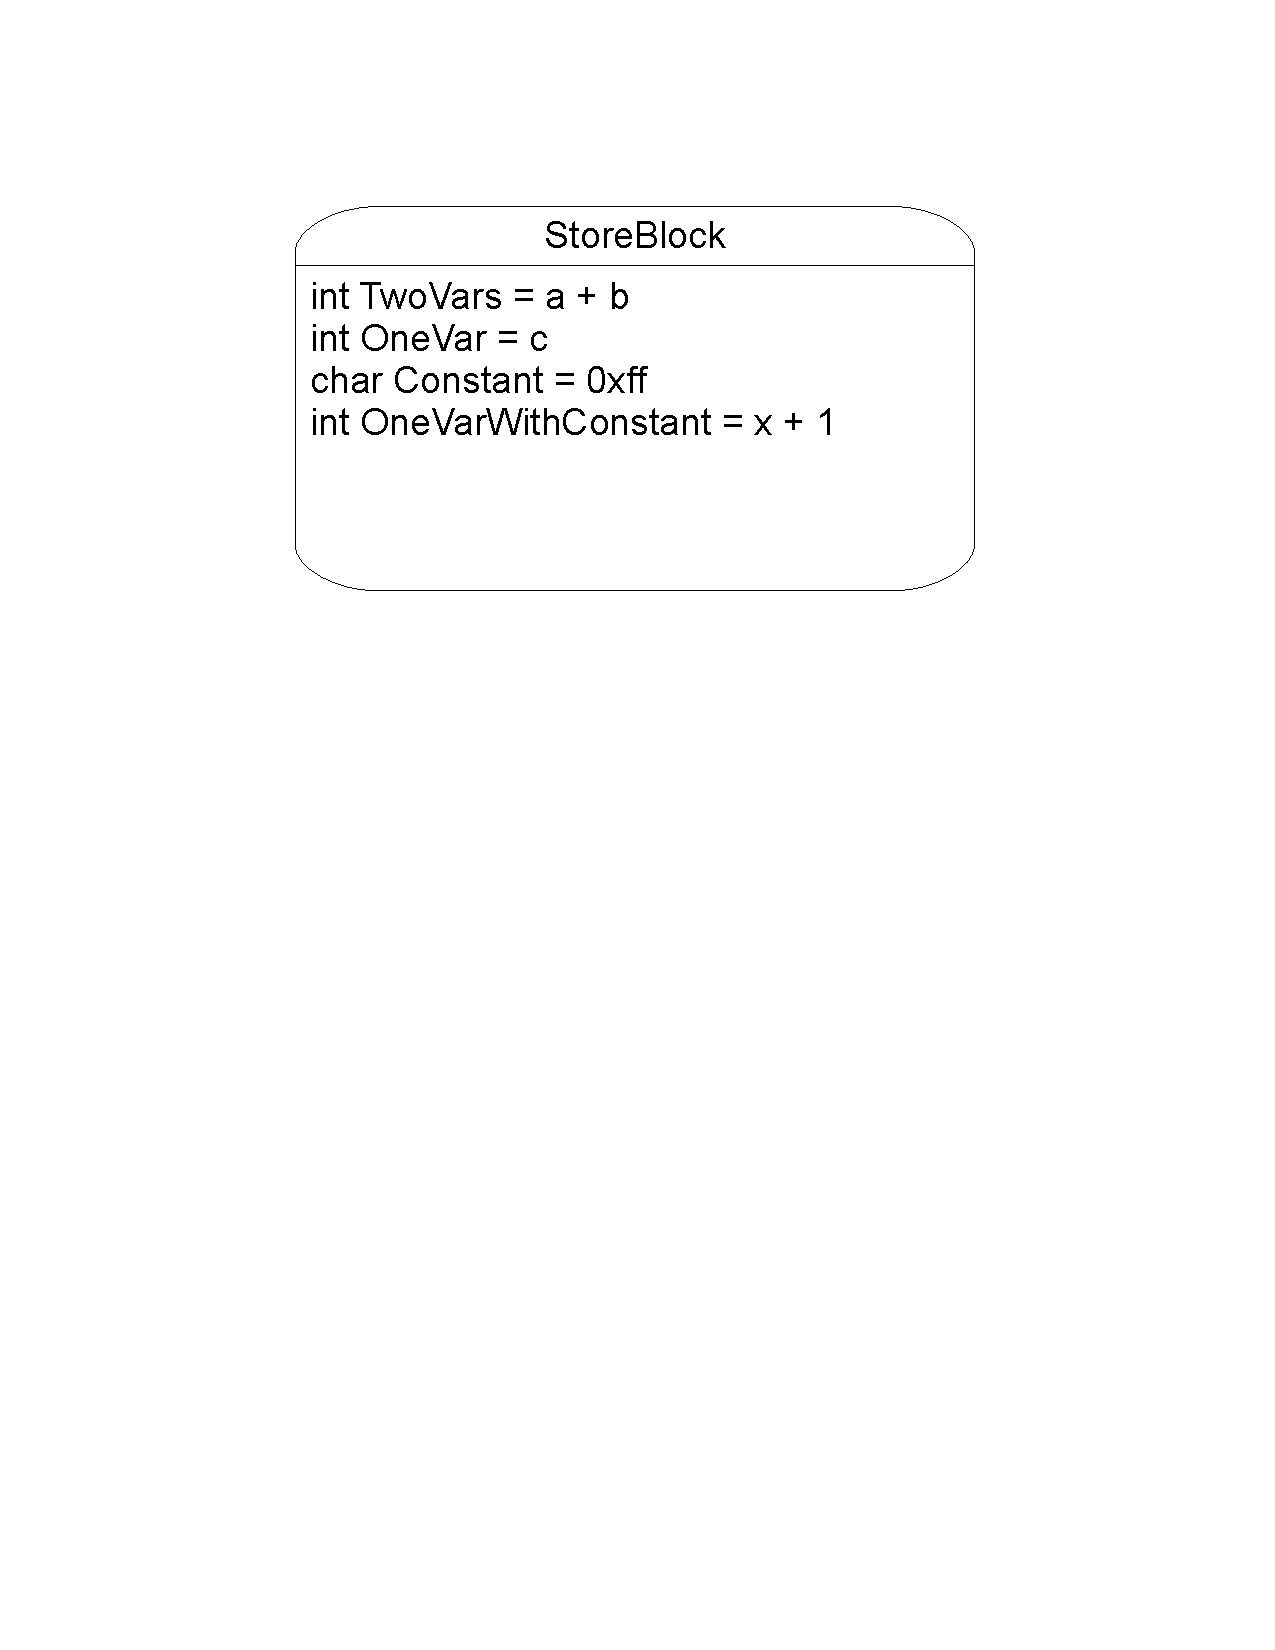
\includegraphics[trim= 20mm 175mm 20mm 10mm, clip, width=\imgmedium]{./images/state_storeblock.pdf}
    \caption{Example Of A Store Block As Implemented In PLCEdit}
    \label{fig:state_storeblock}
\end{figure}

In Figure \ref{fig:state_storeblock} we see a store block represented as it is drawn by the \plcchart $\:$ IDE. Each line consists of a type (can be seen in Figure \ref{fig:state_storeblock} we have \textbf{int}, and \textbf{byte}) an identifier, the equals symbol, and a expression. An expression can take the form of a constant as shown in figure \ref{fig:state_storeblock}. Our syntax also allows for many lines in each StoreBlock. This design choice allows formulae to be expressed more conveniently as it can be done in sequence rather than a sequence of blocks used together to perform a set of operations.
Each of the assignment lines in a store block are read in sequence, and is understood to occur one right after the other. This is described in more detail below.

\begin{align}
v_1 := v_0 \label{eqn:assign0} \\ 
v_0 := v_1 \label{eqn:assign1}
\end{align}

If assignments in \emphasize{\plcchart s} would happen concurrently \ref{eqn:assign0} and \ref{eqn:assign1} would produce a swap where $v'_1 =\: 'v_0$ and $v'_0 =\: 'v_1$ (where $'v$ denotes the value of $v$ before the assignments are made and $v'$ the value of $v$ after the assignment is completed). We read assignments such as in equations \ref{eqn:assign0} and \ref{eqn:assign1} as these assignments will take place upon entry of the mode. For \emphasize{\plcchart s} we read them in a sequential fashion for example: Upon entry of the mode, first equation \ref{eqn:assign0} is assigned, then equation \ref{eqn:assign1}. That is $v'_1 =\: 'v_0$ and then $v'_0 = v'_1$ which results in $v'_0 = v'_1 =\: 'v_0$ after the second assign statement.

\begin{figure}[htp]
    \centering
    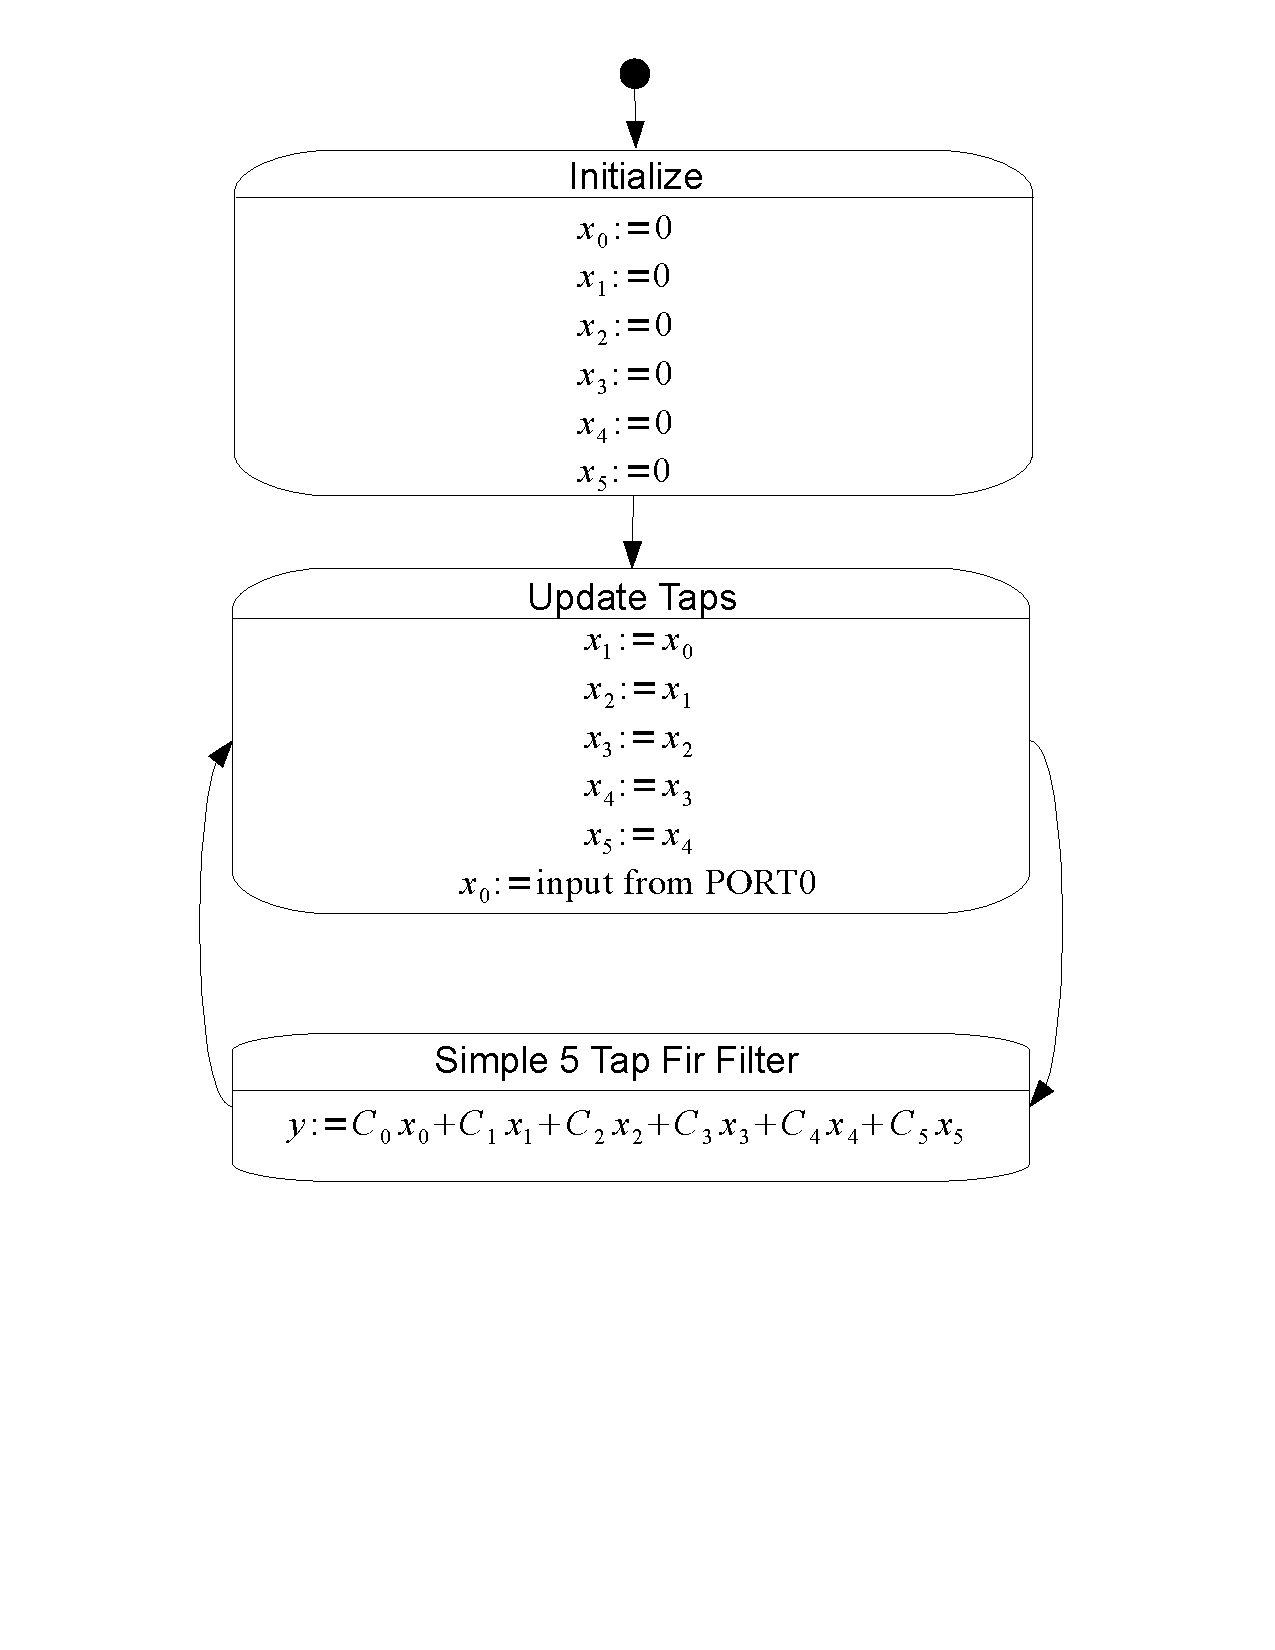
\includegraphics[trim= 10mm 70mm 10mm 10mm, clip, width=250px]{./images/state_uml2_fir.pdf}
    \caption{5 Tap Fir Filtering}
    \label{fig:state_uml2_fir}
\end{figure}

The advantage of sequential assignments over concurrent assignments can be seen when trying to compute a 5 stage fir filter as seen in figure \ref{fig:state_uml2_fir}. In figure \ref{fig:state_uml2_fir} sequential assignments are much more convenient when making many small assignments. Without sequential assignments many more mode blocks would be required to achieve the same behaviour.




